\documentclass[10pt,a4paper]{article}

% Marges du document %
\setlength{\topmargin}{0cm}
\setlength{\headheight}{0.4cm}
\setlength{\headsep}{0.8cm}
\setlength{\footskip}{1cm}
\setlength{\textwidth}{17cm}
\setlength{\textheight}{25cm}
\setlength{\voffset}{-1.5cm}
\setlength{\hoffset}{-0.5cm}
\setlength{\oddsidemargin}{0cm}
\setlength{\evensidemargin}{0cm}

\usepackage{amssymb}
\usepackage{psfrag}
\usepackage[utf8]{inputenc}
\usepackage[francais]{babel}
\usepackage[T1]{fontenc}
\usepackage{amsmath}
\usepackage{amsfonts}
\usepackage{amssymb}
\usepackage{graphicx}
\usepackage{subcaption}
\usepackage{fancyhdr}
\usepackage{multicol}
\usepackage{eurosym} % symbole €
\usepackage{siunitx}
\usepackage{stmaryrd}
\usepackage{bm}

\usepackage{tabu}
\def\€{\euro{}}

\numberwithin{equation}{section}

\newcommand\numberthis{\addtocounter{equation}{1}\tag{\theequation}} 

\usepackage{color} % gestion de différentes couleurs
\definecolor{linkcolor}{rgb}{0,0,0}
\definecolor{linkcolorurl}{rgb}{0,0,1}
\usepackage[ pdftex,colorlinks=true,
pdfstartview=FitV,
linkcolor= linkcolor,
citecolor= linkcolor,
urlcolor= linkcolorurl,
hyperindex=true,
hyperfigures=false]
{hyperref} % fichiers pdf 'intelligents', avec des liens entre les références, etc.

% En-tête et pied de page % 
\pagestyle{fancy}
\fancyhead[L]{\scriptsize \textsc{Chauffage par impact des planétésimaux}} 
\fancyhead[R]{\scriptsize \textsc{BUNEL Félix et VERGNET Hadrien}} 
\fancyfoot[C]{ \thepage}

\author{BUNEL Félix et VERGNET Hadrien}

%%%%%%%%%%%%%%%%%%%%%%%%%%%%%
% Tikz packages and settings
%%%%%%%%%%%%%%%%%%%%%%%%%%%%%

\usepackage{tikz}
\usepackage{pgfplots}
\usepackage{tikz-3dplot}
\pgfplotsset{compat=1.11}

\usetikzlibrary{shapes.geometric,calc,intersections}
\usetikzlibrary{shapes.arrows}
\usetikzlibrary{shadings}
\usetikzlibrary{patterns}
\usetikzlibrary{decorations.pathmorphing}
\usetikzlibrary{decorations.pathreplacing}


\usetikzlibrary{external}
\tikzset{external/aux in dpth={false}}
\tikzset{external/up to date check={simple}}
\tikzset{external/optimize command away={\includetexgraphics}{2}}

\tikzset{>=stealth}

%%%%%%%%%%%%%%%%%%%%%%%%%%%%%%%%%%%%%%%%%%%%%%%%%%%%%%%%%%%%
% Custom macro to input a tikz picture and setting its name
%%%%%%%%%%%%%%%%%%%%%%%%%%%%%%%%%%%%%%%%%%%%%%%%%%%%%%%%%%%%

\makeatletter
\newcommand{\includetikzgraphics}[1]{
	\filename@parse{#1}
	\tikzsetnextfilename{\filename@base}
	\input{#1}
}
\makeatother

%%%%%%%%%%%%%%%%%%%%%%%%%%%%%%%%%%
% Custom tikz command for drawing
%%%%%%%%%%%%%%%%%%%%%%%%%%%%%%%%%%

\tikzset{math3d/.style=
    {z= {(-0cm,-0.3cm)}, y={(0cm,1cm)},x={(1cm,0cm)}}}

% \drawYNema {x} {y} {yAngle}
\newcommand{\drawYnema}[3] {
	\shade [ball color=black] (#1,#2) ellipse 
		[x radius={sqrt(pow(cos(#3)*0.1,2)+pow(sin(#3)*0.3,2))}, y radius=0.1];
}
% \drawXNema {x} {y} {xAngle}
\newcommand{\drawXnema}[3] {
	\shade [ball color=black] (#1,#2) ellipse 
		[y radius={sqrt(pow(cos(#3)*0.1,2)+pow(sin(#3)*0.3,2))}, x radius=0.1];
}
% \drawZNema {x} {y} {zAngle}
\newcommand{\drawZnema}[3] {
	\shade [ball color=black] (#1,#2) ellipse 
		[x radius=0.3, y radius=0.1, rotate={#3}];
}

% \plotcylinder { radius } { heigth } { altitude }
\newcommand{\plotcylinder}[3] {
     \draw [math3d, fill=white, samples=100]
        plot[domain=-pi:pi] ({#1*cos(\x r)},#3,{#1*sin(\x r)}) ;
     \draw [math3d, fill=white, samples=100]
        plot[domain=0:pi] ({#1*cos(\x r)},#3,{#1*sin(\x r)}) --
        plot[domain=pi:0] ({#1*cos(\x r)},{#3-#2},{#1*sin(\x r)}) --
        cycle;
}

% \plotpolarizer { x} { y} { z } { radius } { angle }
\newcommand{\plotpolarizer}[5] {
    \draw [math3d, fill=gray, opacity=0.8, samples=100]
        plot[domain=-pi:pi] ({#1+#4*cos(\x r)},#2,{#3+#4*sin(\x r)}) ;
    \draw [math3d, opacity=0.8]
        ({#1+#4*cos(#5)},#2,{#3+#4*sin(#5)}) -- ({#1-#4*cos(#5)},#2,{#3-#4*sin(#5)}) ;
}

% \fancyarrow {xi} {yi} {xf} {yf} {width} {options}
\newcommand{\fancyarrow}[6]{
	\pgfmathsetmacro{\dx}{#3-#1};
	\pgfmathsetmacro{\dy}{#4-#2};
	\pgfmathsetmacro{\dl}{sqrt(\dx*\dx+\dy*\dy)};
	\pgfmathsetmacro{\dw}{#5/2};
	\pgfmathsetmacro{\cos}{\dx/\dl};
	\pgfmathsetmacro{\sin}{\dy/\dl};
	\draw [#6] (#1,#2) -- ++($\dw*(\sin,-\cos)$) 
		-- ++(${\dl-2*\dw}*(\cos,\sin)$)
		-- ++($\dw*(\sin,-\cos)$) -- ++($2*\dw*(\cos,\sin)+2*\dw*(-\sin,\cos)$) 
		-- ++($-2*\dw*(\cos,\sin)+2*\dw*(-\sin,\cos)$) -- ++($\dw*(\sin,-\cos)$)
		-- ++(${2*\dw-\dl}*(\cos,\sin)$) -- cycle;
}

%%%%%%%%%%%%%%%%%%%%%%%
% Custom pgf mark list
%%%%%%%%%%%%%%%%%%%%%%%
\pgfplotscreateplotcyclelist{colorhollowmarks}{%
	{black,mark=x},
	{cyan,mark=+},
	{magenta,mark=o},
	{teal,mark=square},
	{violet,mark=triangle},
	{gray,mark=diamond},
	{brown,mark=pentagon},
	{orange,mark=otimes},
	{lime,mark=10-pointed star}}
\pgfplotscreateplotcyclelist{hollowmarks}{%
	{mark=x},
	{mark=+},
	{mark=o},
	{mark=square},
	{mark=triangle},
	{mark=diamond},
	{mark=pentagona},
	{mark=otimes},
	{mark=10-pointed star}}
\pgfplotscreateplotcyclelist{onlycolors}{%
	black,
	cyan,
	magenta,
	teal,
	violet,
	lightgray,
	brown,
	orange,
	lime}



\begin{document}

%%%%%%%%%%%%%%%%%%%%%%%%%%%%%%%%%%%%%%%%%%%%%%%%%%%%%%%%%%%%%%%%%%%%%%%%%%%%%%%%%%%%%%%%
%%%%%%%%%%%%%%%%%%%%%%%%%%%%%%%%%%%%%%%%%%%%%%%%%%%%%%%%%%%%%%%%%%%%%%%%%%%%%%%%%%%%%%%%
\begin{titlepage}
%%%%%%%%%%%%%%%%%%%%%%%%%%%%%%%%%%%%%%%%%%%%%%%%%%%%%%%%%%%%%%%%%%%%%%%%%%%%%%%%%%%%%%%%
%%%%%%%%%%%%%%%%%%%%%%%%%%%%%%%%%%%%%%%%%%%%%%%%%%%%%%%%%%%%%%%%%%%%%%%%%%%%%%%%%%%%%%%%
\thispagestyle{empty}
\setlength{\parindent}{0pt}


\includegraphics[height=1.9cm]{logo-ens.jpg} \hfill 
\includegraphics[height=2cm]{logo_lyon1.jpg} \hfill 
\includegraphics[height=2cm]{logo_univ_lyon.jpg}



Master Sciences de la matière
\hfill
Projet de Géophysique

\textit{École Normale Supérieure de Lyon}
\hfill
BUNEL Félix et VERGNET Hadrien

\textit{Université Claude Bernard Lyon 1}
\hfill
M2 Physique 2016-2017
\vspace{0.5cm}

\hrulefill
\vspace{-0.6cm}

\hrulefill
\begin{center}\bfseries
\vspace{0.4cm}

\begin{huge}
	Chauffage par impact des planétésimaux    
\end{huge}
\vspace{0.5cm}

Rapport de Félix Bunel. Projet réalisé avec Hadrien Vergnet
\end{center}
\hrulefill
\vspace{-0.6cm}

\hrulefill


\begin{center}
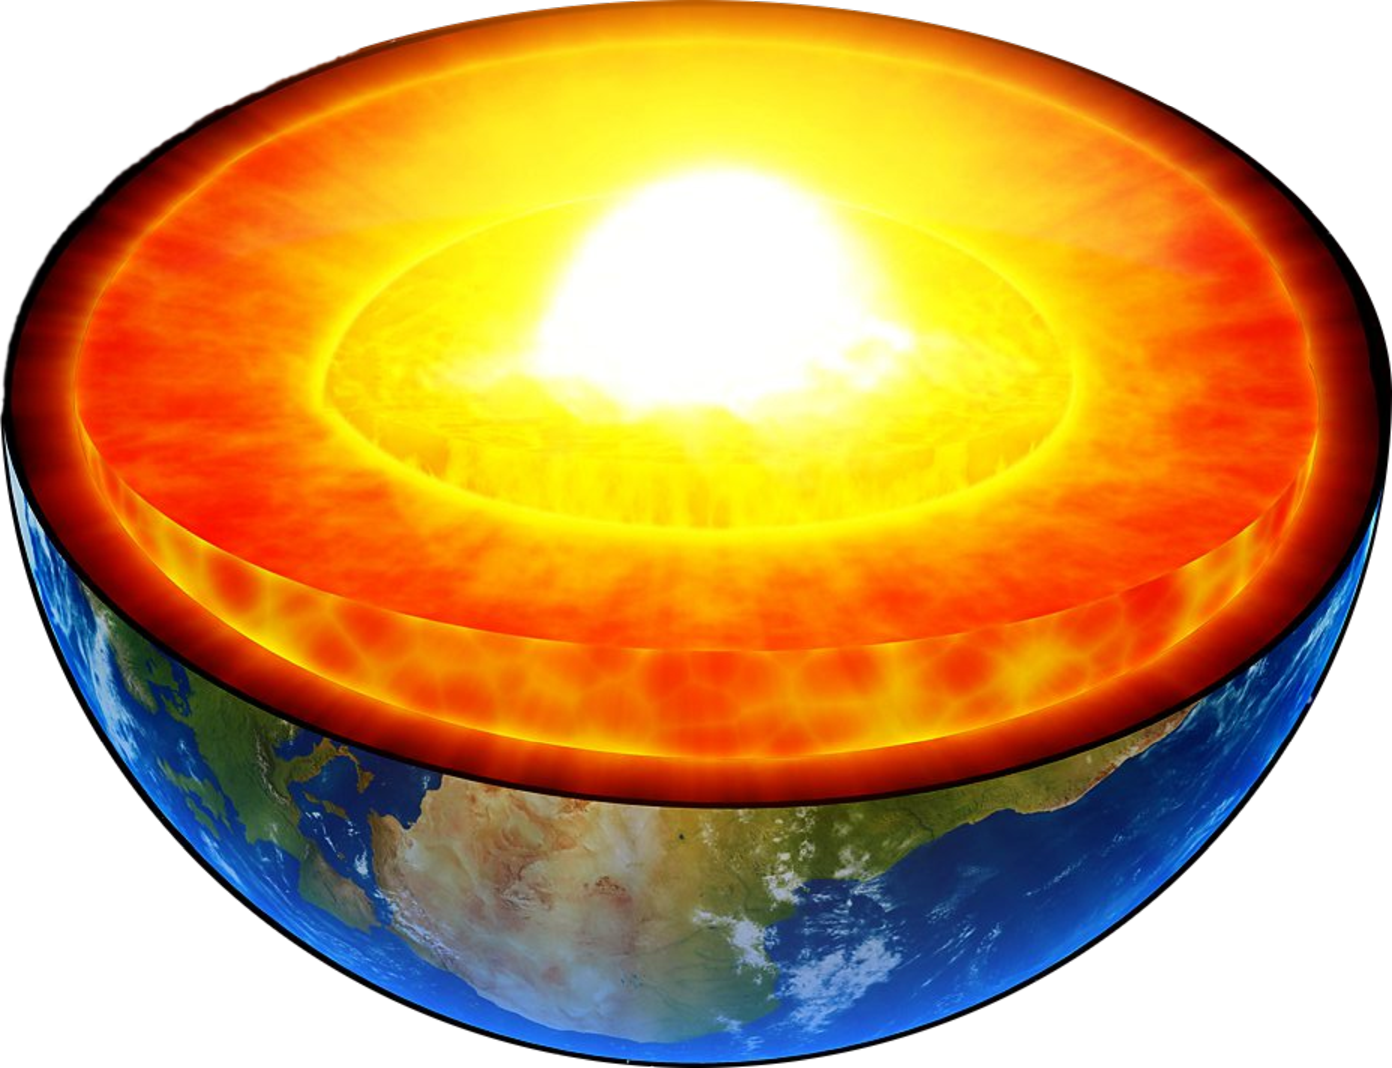
\includegraphics[height=5cm]{figures/terre_core.pdf} 
\end{center} 


\textbf{Résumé :} Le projet réalisé s'intéresse à l'évolution en température d'un planétésimal afin d'étudier l'importance du chauffage par impact dans la différentiation. 
On montre à l'aide de plusieurs modèles de complexité croissante que le chauffage par impact n'est pas le facteur permettant une formation rapide d'un noyau métallique.
Ce projet s'inspire grandement de l'article \textit{Thermal evolution and differentiation of planetesimals and planetary embryos. (2012), Icarus, 217(1), 339-354.} par Šrámek, O., Milelli, L., Ricard, Y., et Labrosse, S. . 



\vspace{0.3cm}

\textbf{Mots clefs :} planétésimaux, diffusion, accrétion.
\vspace{0.3cm}


\tableofcontents

\end{titlepage}

\newpage
\renewcommand\thepage{\arabic{page}}


\setcounter{page}{1}


\definecolor{linkcolor}{rgb}{0,0,1}

%%%%%%%%%%%%%%%%%%%%%%%%%%%%%%%%%%%%%%%%%%%%%%%%%%%%%%%%%%%%%%%%%%%%%%%%%%%%%%%%%%%%%%%%
%%%%%%%%%%%%%%%%%%%%%%%%%%%%%%%%%%%%%%%%%%%%%%%%%%%%%%%%%%%%%%%%%%%%%%%%%%%%%%%%%%%%%%%

\section*{Introduction}
%%%%%%%%%%%%%%%%%%%%%%%%%%%%%%%%%%%%%%%%%%%%%%%%%%%%%%%%%%%%%%%%%%%%%%%%%%%%%%%%%%%%%%%%
%%%%%%%%%%%%%%%%%%%%%%%%%%%%%%%%%%%%%%%%%%%%%%%%%%%%%%%%%%%%%%%%%%%%%%%%%%%%%%%%%%%%%%%%
\addcontentsline{toc}{section}{Introduction}

La formation de notre système solaire est encore aujourd'hui un mystère qui suscite de nombreuses recherches. Le mécanisme ayant permis l'évolution d'un nuage de poussières vers les planètes que l'on connaît aujourd'hui est encore mal compris. 
\medskip

Les grandes lignes de ce mécanisme sont bien connues. La poussière autour du soleil va coalescer et former des corps de quelques kilomètres de diamètre. Ces embryons de planètes appelés planétésimaux, attirent ensuite la matière environnante ainsi que des planétésimaux plus petits et évoluent finalement vers les planètes telles que nous les connaissons.
Cependant, les détails de ces mécanismes sont encore à préciser. Des preuves récentes montrent par exemple que la séparation des astres en un noyau métallique liquide et un manteau solide composé de silicates se serait faite très tôt dans l'histoire de ces planètes. Les mécanismes permettant cette différentiation rapide au niveau des planétésimaux reste une question ouverte de la recherche actuelle. 
\medskip

Dans ce rapport, on s'intéresse justement à ces mécanismes de différentiation. Plus précisément, l'objectif est d'étudier, par une étude de diffusion thermique simple, la différentiation dans les planétésimaux. En comparant les profils de températures à l'intérieur d'un planétésimal aux températures de fusion des éléments présents, il est possible de déterminer si oui ou non la fusion est possible. La présence de cette fusion pourrait en effet expliquer les différentiations rapides observées par des mécanismes de percolation ou simplement de séparation de phase. 
L'originalité de ce projet réside dans l'étude de l'influence de différents termes de chauffage dans l'équation de la chaleur. En plus d'un terme de chauffage radioactif généralement utilisé dans ce genre d'étude, on a considéré un terme de chauffage par impact couplé à l'évolution en taille du planétésimal.
\medskip

La résolution de ce problème a été réalisée numériquement. Pour résumer, on a résolu l'équation de la chaleur en géométrie sphérique par des différences finies. Les méthodes numériques ainsi que les détails du modèle physique employés sont décrits dans la première partie de ce rapport. Ensuite, une seconde partie présente les résultats obtenus pour une planète de taille constante. Une troisième partie présente l'influence de la croissance de la planète sur les profils de températures observées. Enfin, l'implémentation du chauffage par impact ainsi que son importance dans le chauffage des planétésimaux sont discutés dans une dernière partie.

%%%%%%%%%%%%%%%%%%%%%%%%%%%%%%%%%%%%%%%%%%%%%%%%%%%%%%%%%%%%%%%%%%%%%%%%%%%%%%%%%%%%%%%%
%%%%%%%%%%%%%%%%%%%%%%%%%%%%%%%%%%%%%%%%%%%%%%%%%%%%%%%%%%%%%%%%%%%%%%%%%%%%%%%%%%%%%%%%
\section{Modèle et méthodes numériques}
%%%%%%%%%%%%%%%%%%%%%%%%%%%%%%%%%%%%%%%%%%%%%%%%%%%%%%%%%%%%%%%%%%%%%%%%%%%%%%%%%%%%%%%%
%%%%%%%%%%%%%%%%%%%%%%%%%%%%%%%%%%%%%%%%%%%%%%%%%%%%%%%%%%%%%%%%%%%%%%%%%%%%%%%%%%%%%%%%
\subsection{Modèle théorique}

On cherche donc à étudier l'évolution d'un planétésimal. Pour cela, plusieurs hypothèses simplificatrices ont été réalisées. 
\medskip

Tout d'abord, on ne tient compte que des effets de diffusion. Le planétésimal est modélisé par un mélange homogène constitué de $18\%$ de métal à et de $82\%$ silicates. La séparation de phase n'est donc pas prise en compte. De même les variations des propriétés du mélange avec la température sont négligées. Les constantes du mélanges sont simplement calculées par la moyenne des constantes du métal et des silicates avec des poids associés à leur proportion. Les valeurs des constantes obtenues sont retranscrites en table \ref{constantes}.
\medskip

Utiliser un tel modèle où l'on ne considère qu'un mélange alors que l'on souhaite justement expliquer la différentiation peut sembler inapproprié. Cependant, si l'on considère que la séparation du métal des silicates ne peut se faire que sous forme liquide notre approche reste valide et permet de répondre à la question : est-il possible d'atteindre la température de fusion dans le mélange solide ce qui permettrait une différentiation sous forme liquide ultérieurement ? 
\medskip

Les transitions de phase du métal et des silicates sont prises en compte par l'intermédiaire d'une chaleur latente de changement d'état qui apparaît donc comme une énergie libérée là où il y a solidification et absorbée au niveau de la fusion. L'influence de cette chaleur latente est détaillée en partie \ref{latente}.

\tabulinesep=0.3mm
\begin{table}[h!]
  \center
  \begin{tabu}{ r | c c c l}
     & moyenne & métal & silicate & unité\\ \hline
    Densité ($\rho$) & 4028 & 7800 &  3200 & \SI{}{kg.m^{-3}}\\ \hline
    Capacité calorifique ($C_p$) & 939 & 450 & 1200 &  \SI{}{J.K^{-1}.kg^{-1}} \\ \hline
    Conductivité ($k_T$)& 11.48 & 50 & 3 & \SI{}{W.K^{-1}.m^{-1}}  \\ \hline    
    Chaleur latente de fusion & 413 & 250 & 500 & \SI{}{kJ.kg^{-1}}\\ \hline
    Température de fusion & & 1261 & 1408 & \SI{}{K}\\ \hline
  \end{tabu}
  \caption{Valeur des constantes utilisées pour le modèle.}
  \label{constantes}
\end{table}

Enfin, on a considéré que le problème avait une symétrie sphérique, c'est à dire que les variations de température ne dépendent que de la coordonnée radiale. Sous ces hypothèses, notre planétésimal est régit simplement par une équation de la diffusion en sphérique :
\begin{equation}
\rho C_p \dfrac{\partial T}{\partial t} = \frac{k_{T}}{r^2} \dfrac{\partial }{\partial r}\left( r^2 \dfrac{\partial T}{\partial r} \right) + P
\label{diffusion}
\end{equation}
où $r$ est la coordonnée radiale, $T$ la température et $P$ un terme de production de chaleur.
\medskip

Le terme de production comprend tout d'abord le chauffage radioactif $P_{rad}$ dû à la décomposition des éléments radioactifs présents. Dans cette étude, on considère uniquement le chauffage dû à l'aluminium 26. Bien entendu, l'amplitude de ce terme décroît de manière exponentielle avec le temps. Il est sous la forme :
\begin{equation}
P_{rad} = P_{0}2^{-t/\tau_{1/2}}
\end{equation}
où $P_{0}$ est le chauffage initial et $\tau_{1/2}$ le temps de demi-vie de l'aluminium 26 qui est de 0.717 My. Le chauffage initial peut être calculé à l'aide de l'abondance en aluminium 26 à l'intérieur du planétésimal et a été estimé à \SI{1.5E-7}{W.kg^{-1}}.
Le terme de production comprend également les pertes à la surface qui ont été prises comme le rayonnement d'un corps noir à la température de la surface.
Enfin, ce terme comprend également le chauffage par impact dû aux impactants. Le détail de ce terme sera développé en partie \ref{impactant}.
\medskip

La dernière chose à préciser est la question de la condition initiale. Une des possibilités est de considérer que le planétésimal s'est formé presque instantanément à partir d'un nuage de poussière. De sorte, la température initiale du planétésimal est essentiellement dûe à la température de la nébuleuse soit 300 K. L'autre source d'énergie pouvant augmenter la température initiale est bien entendu l'énergie gravitationnelle récupérée lors de l'effondrement du nuage de poussière. Cette énergie peut être calculée analytiquement et vaut :
\begin{equation}
E_{G} = \frac{3}{5}\frac{GM}{R^2}
\end{equation}
où $M$ est la masse et $R$ le rayon du planétésimal. Cette énergie introduit un surplus de température par rapport à la température de la nébuleuse qui vaut :
\begin{equation}
\Delta T = \frac{4 \pi}{5}\frac{\rho G}{C_p}R^2
\end{equation}
Cependant, pour le rayon initial de 5 km utilisé dans toute cette étude, cette énergie n'est que de 0.02 K et peut donc être négligée devant la température de la nébuleuse.


\subsection{Résolution numérique}

On souhaite résoudre l'équation de la chaleur sphérique numériquement. 
\medskip

Pour cela, la première des étapes est d'adimensionner les équations pour limiter les erreurs numériques. Une bonne échelle temporelle est bien évidement le temps de demi-vie de l'aluminium 26 $\tau_{1/2}$ qui est le temps caractéristique de notre modèle. \`A partir de ce temps, il est possible de créer une longueur de diffusion à l'aide de la conductivité thermique $L_d = \sqrt{\frac{k_T \tau_{1/2}}{\rho C_p} } \simeq 10$ km. Enfin, une bonne température de référence est celle de la nébuleuse $T_{neb}$.
En injectant ces variables dans l'équation de diffusion \ref{diffusion}, on obtient en unités adimensionnées :
\begin{equation}
\dfrac{\partial T}{\partial t} = \frac{1}{r^2} \dfrac{\partial }{\partial r}\left( r^2 \dfrac{\partial T}{\partial r} \right) + c_0P
\label{diffusion_adim}
\end{equation}
avec 
\begin{equation}
c_0 = \frac{\tau_{1/2}}{\rho C_p T_{neb}}
\end{equation}

L'équation a ensuite été discrétisée tant dans le domaine temporel que spatial. La discrétisation sur la coordonnée radiale se fait sur un maillage uniforme de pas $\Delta r$ à l'aide d'un schéma d'Euler centré. Le laplacien est alors donné par :
\begin{align}
\frac{1}{r^2} \dfrac{\partial }{\partial r}\left( r^2 \dfrac{\partial T}{\partial r} \right) &\rightarrow \frac{1}{r^2_i \Delta r}\left[ r^2_{i+1/2}\frac{T_{i+1} - T_{i}}{\Delta r} + r^2_{i-1/2}\frac{T_{i-1} - T_{i}}{\Delta r} \right]
\end{align}
Les variations temporelles sont quant à elles décrites à l'aide d'un schéma d'Euler implicite.
\medskip

En pratique, résoudre un pas de temps revient donc à résoudre un système de la forme :
\begin{equation}
MT^{t+1} = T^t + c_0 P^{t}
\end{equation}
Avec la matrice $$M = \left[ Id + \frac{\Delta t ~ r^2_{i+1/2}}{r^2_i \Delta r^2} ~ d1 + \frac{\Delta t ~ r^2_{i-1/2}}{r^2_i \Delta r^2} ~ d2  \right]$$
où $d_1$ et $d_2$ sont des matrices sur et sous diagonales supérieures et inférieures. $M$ est donc une matrice tridiagonale.
$$
d1=
\begin{bmatrix}
    2      & -1     & -1       &   \\
           &  1     & -1              &             \\
     &        & \ddots    &\ddots       \\
     &        &            & 1 & -1         \\
         &   &      &   0         &  0
\end{bmatrix}
\qquad
d2=
\begin{bmatrix}
     0     & 0      &   &     &        \\
    -1     & 1      &  &          &            \\
     & \ddots & \ddots &    &      \\
     &              &  -1      &  1         \\
         &      &  -1     & -1        & 2 \\
\end{bmatrix}
$$

%%%%%%%%%%%%%%%%%%%%%%%%%%%%%%%%%%%%%%%%%%%%%%%%%%%%%%%%%%%%%%%%%%%%%%%%%%%%%%%%%%%%%%%%
%%%%%%%%%%%%%%%%%%%%%%%%%%%%%%%%%%%%%%%%%%%%%%%%%%%%%%%%%%%%%%%%%%%%%%%%%%%%%%%%%%%%%%%%
\section{Influence du chauffage et de la chaleur latente}
%%%%%%%%%%%%%%%%%%%%%%%%%%%%%%%%%%%%%%%%%%%%%%%%%%%%%%%%%%%%%%%%%%%%%%%%%%%%%%%%%%%%%%%%
%%%%%%%%%%%%%%%%%%%%%%%%%%%%%%%%%%%%%%%%%%%%%%%%%%%%%%%%%%%%%%%%%%%%%%%%%%%%%%%%%%%%%%%%
On s'intéresse dans un premier temps à l'évolution en température d'un corps de taille fixe chauffé uniquement par le chauffage radioactif. Les profils de température observés seront donc le résultat de l'équilibre entre le chauffage radioactif et les pertes de chaleur à la surface.

\subsection{Régimes d'évolution}

Tout d'abord, il est possible de s'intéresser au profil de température dans le planétésimal. Bien entendu, les résultats dépendront du seul paramètre non fixé de ce modèle qui est la taille de l'astre. La figure \ref{diffusion2} représente les profils obtenus pour différentes tailles d'astres. 

\begin{figure}[h]
    \centering	    
	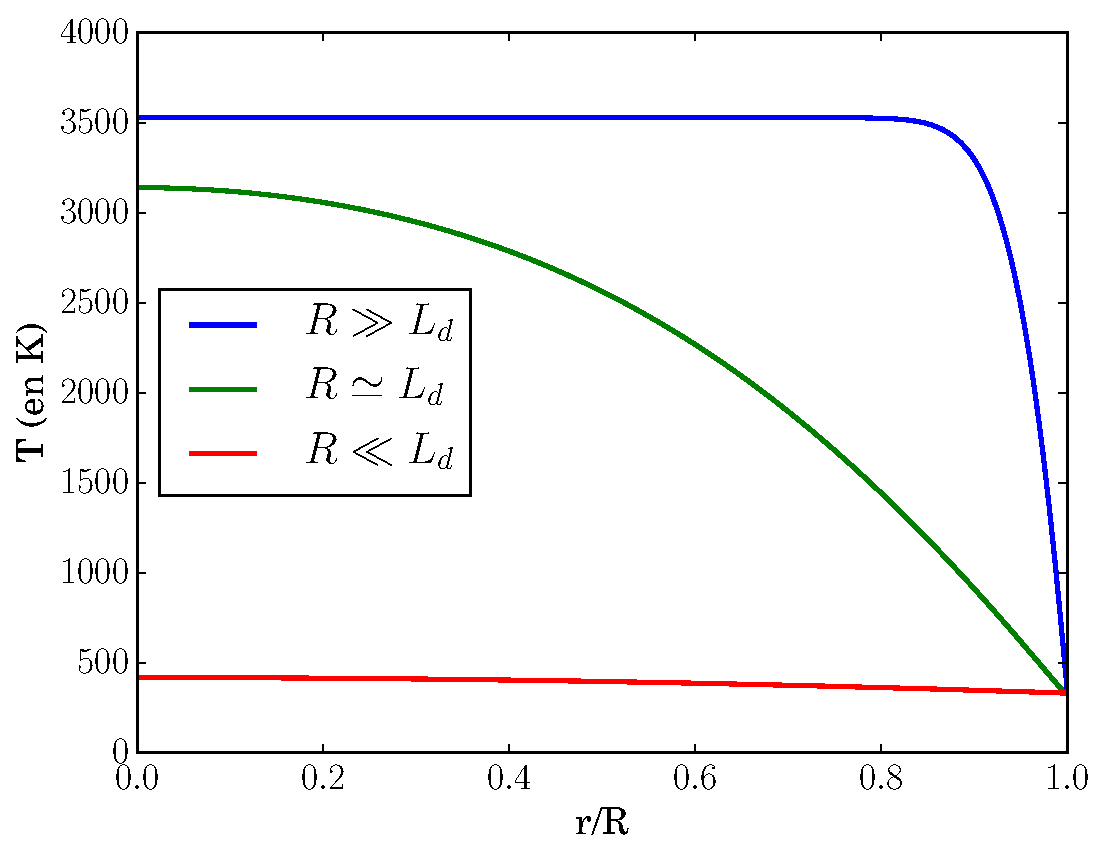
\includegraphics[scale=0.43]{figures/diffusion2.pdf}
    \caption{Profil de température après 1 My pour différents rayons : $R= 2$, $20$ et $200$ km. }
    	\label{diffusion2} 
\end{figure}

La première chose à remarquer sur cette figure est que la température à la surface est toujours très proche de la température de la nébuleuse. Le rayonnement du corps noir est en effet extrêmement efficace pour évacuer la chaleur. 
\medskip

Ensuite, on peut voir que 3 régimes suivant le rayon sont observés. Lorsque le rayon est faible devant la longueur de diffusion, les effets de la diffusion sont très importants de sorte que toute la chaleur générée par la radioactivité est rapidement diffusée vers la surface. La température de l'astre est donc relativement uniforme et proche de celle de la nébuleuse. Pour des rayons grands devant la longueur de diffusion, la température à l'intérieure est beaucoup plus élevée puisque l'énergie créée n'a pas le temps d'être diffusée à la surface. La température est donc constante en dehors de la surface ou la température est fixée par le rayonnement. Pour des rayons proches de la longueur de diffusion un comportement intermédiaire est observé où la température augmente avec la profondeur.

\newpage
\subsection{Chaleur latente de changement d'état}
\label{latente}

Il est également possible de s'intéresser à l'importance de la chaleur latente de changement d'état en comparant les profils de température lorsqu'on la considère et lorsqu'elle est négligée.

\begin{figure}[h]
    \centering	    
	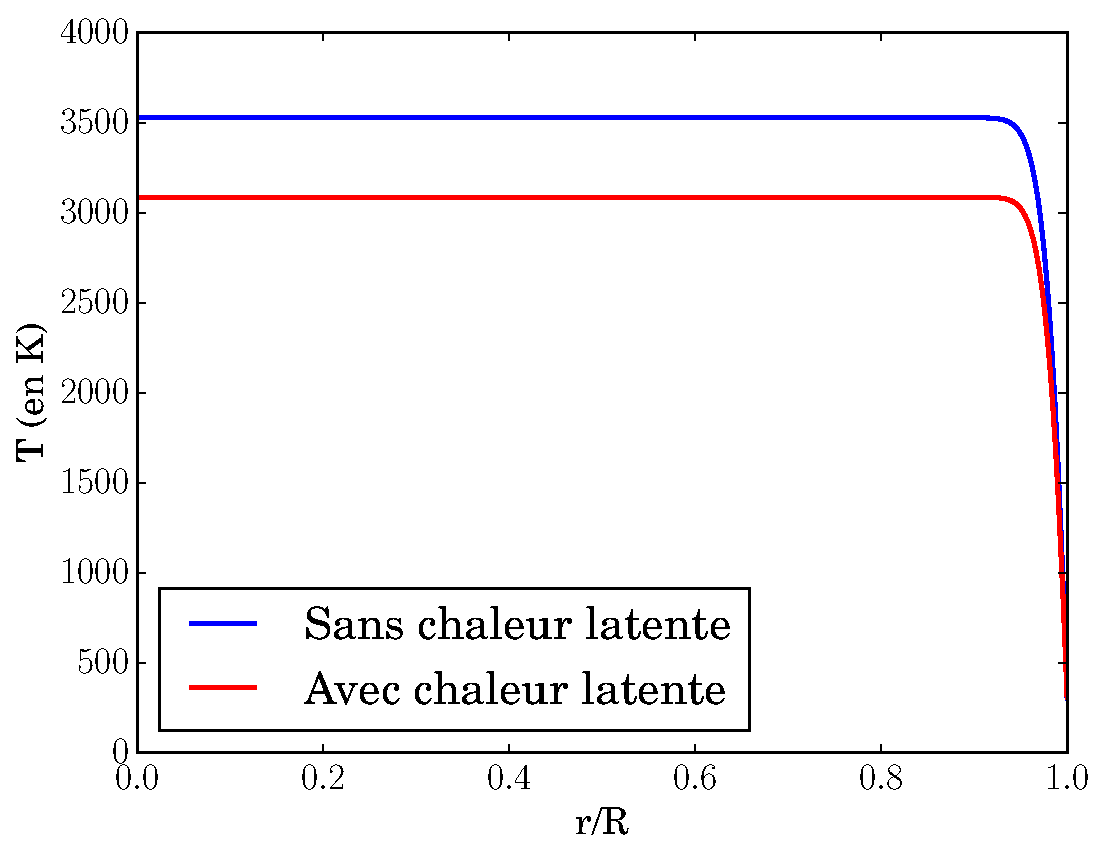
\includegraphics[scale=0.43]{figures/diffusion1.pdf}
    \caption{Profil de température après 1 My pour un rayon de 500 km avec et sans chaleur latente.}
    	\label{diffusion1} 
\end{figure}
\medskip

Comme on peut le voir en figure \ref{diffusion1}, un décalage de 300 K entre le cas avec et sans chaleur latente est observé. En effet, ce décalage s'explique par l'énergie qui a été nécessaire pour réaliser la fusion. On peut dire que cette énergie est stockée dans l'état liquide et pourra être libérée si il y a solidification.

\subsection{Température moyenne au cours du temps}
Enfin, la dernière chose que l'on peut vérifier avec ce modèle est l'évolution temporelle logique d'un tel astre. Au début de sa vie, le chauffage radioactif est suffisamment important pour augmenter sa température. Après un temps supérieur à quelque fois le temps de demi-vie ce chauffage n'est cependant plus très efficace et la température de l'astre diminue à cause des pertes à la surface. La figure \ref{tempMoy} représente une telle évolution en fonction du temps.
\begin{figure}[h]
    \centering	    
	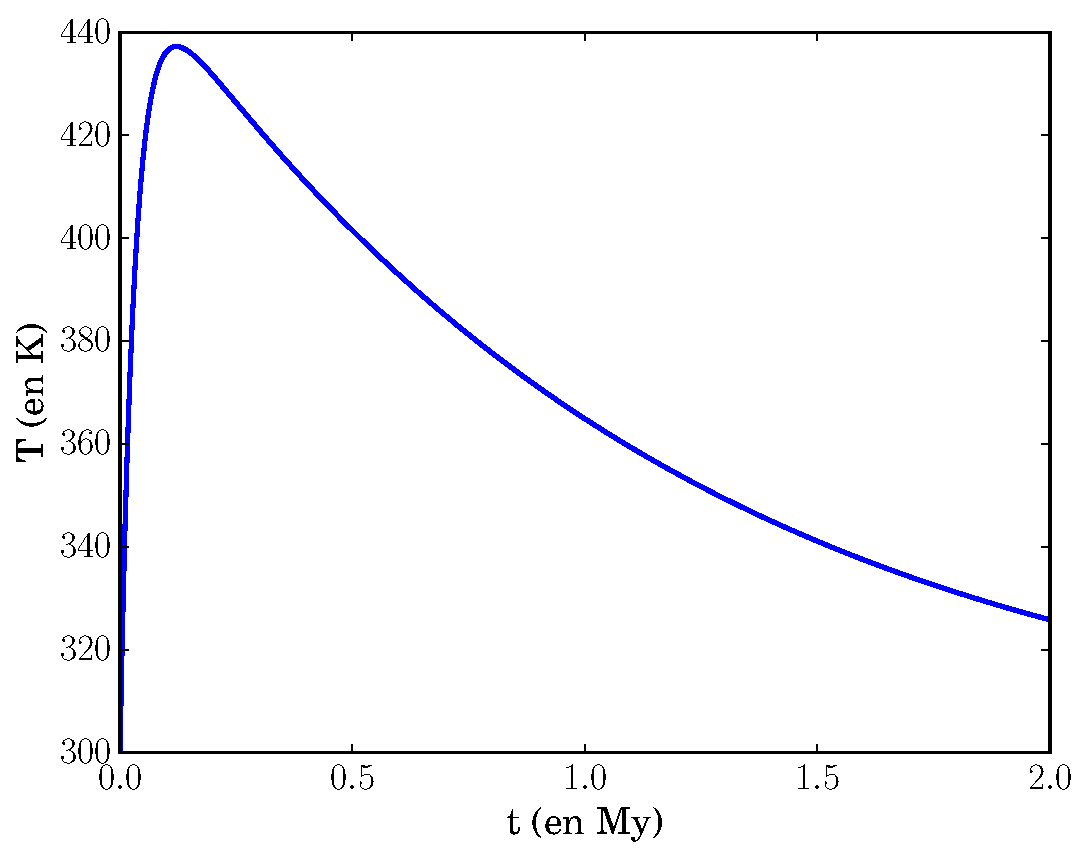
\includegraphics[scale=0.43]{figures/tempMoy.pdf}
    \caption{Température moyenne en fonction du temps pour un rayon de 5 km.}
    	\label{tempMoy} 
\end{figure}

\newpage
%%%%%%%%%%%%%%%%%%%%%%%%%%%%%%%%%%%%%%%%%%%%%%%%%%%%%%%%%%%%%%%%%%%%%%%%%%%%%%%%%%%%%%%%
%%%%%%%%%%%%%%%%%%%%%%%%%%%%%%%%%%%%%%%%%%%%%%%%%%%%%%%%%%%%%%%%%%%%%%%%%%%%%%%%%%%%%%%%
\section{Influence d'un terme d'accrétion}
%%%%%%%%%%%%%%%%%%%%%%%%%%%%%%%%%%%%%%%%%%%%%%%%%%%%%%%%%%%%%%%%%%%%%%%%%%%%%%%%%%%%%%%%
%%%%%%%%%%%%%%%%%%%%%%%%%%%%%%%%%%%%%%%%%%%%%%%%%%%%%%%%%%%%%%%%%%%%%%%%%%%%%%%%%%%%%%%%
%%%%%%%%%%%%%%%%%%%%%%%%%%%%%%%%%%%%%%%%%%%%%%%%%%%%%%%%%%%%%%%%%%%%%%%%
\subsection{Forme de l'accrétion}

On considère maintenant une augmentation du rayon de la planète avec le temps. La croissance est supposée suivre une loi de la forme 
\begin{equation}
\dot{R} \propto R^\beta
\end{equation}
en prenant $\beta =$ 0, 1,  où 2. Dans toutes les simulations réalisées, le planétésimal évolue en suivant cette loi de 5 à 500 km en 1 My. La taille du planétésimal en fonction du temps est représenté en figure \ref{rayon}.

\begin{figure}[h]
    \centering	    
	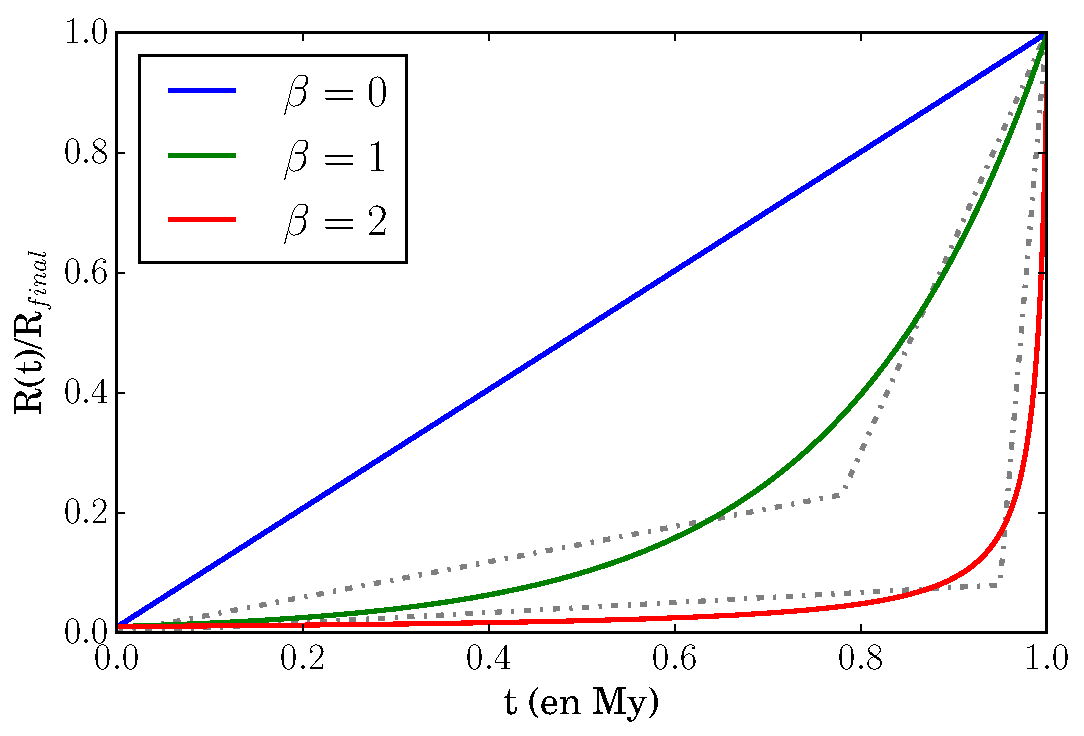
\includegraphics[scale=0.43]{figures/rayon.pdf}
    \caption{Taille du planétésimal en fonction du temps pour différents $\beta$. Les tracés en pointillés correspondent à une simplification des profils en deux régimes.}
    	\label{rayon} 
\end{figure}

Le profil est parfaitement linéaire pour $\beta = 0$. Pour les autres exposants $\beta = 1$ et 2, la croissance se fait plus tardivement : la croissance est lente au début de l'évolution puis croît rapidement vers la fin. Ce rayon variable doit être pris en compte dans les équations ce qui entraîne l'apparition d'un terme qui s'assimile à un terme de transport vers l'intérieur de la planète. Une fois adimensionnée comme précédemment, on obtient l'équation :
\begin{equation}
\dfrac{\partial T}{\partial t} - \dot{R} \dfrac{\partial T}{\partial r} = \frac{1}{r^2} \dfrac{\partial }{\partial r}\left( r^2 \dfrac{\partial T}{\partial r} \right) + c_0P
\label{accretion_adim}
\end{equation}
En pratique, les longueurs sont adimensionnées par rapport au rayon du planétésimal qui évolue avec le temps.

\subsection{Profil de température}

On peut réitérer l'étude précédente en prenant en compte ce terme d'accrétion. La figure \ref{profilacre} représente les profils obtenus.

\begin{figure}[h]
    \centering	    
	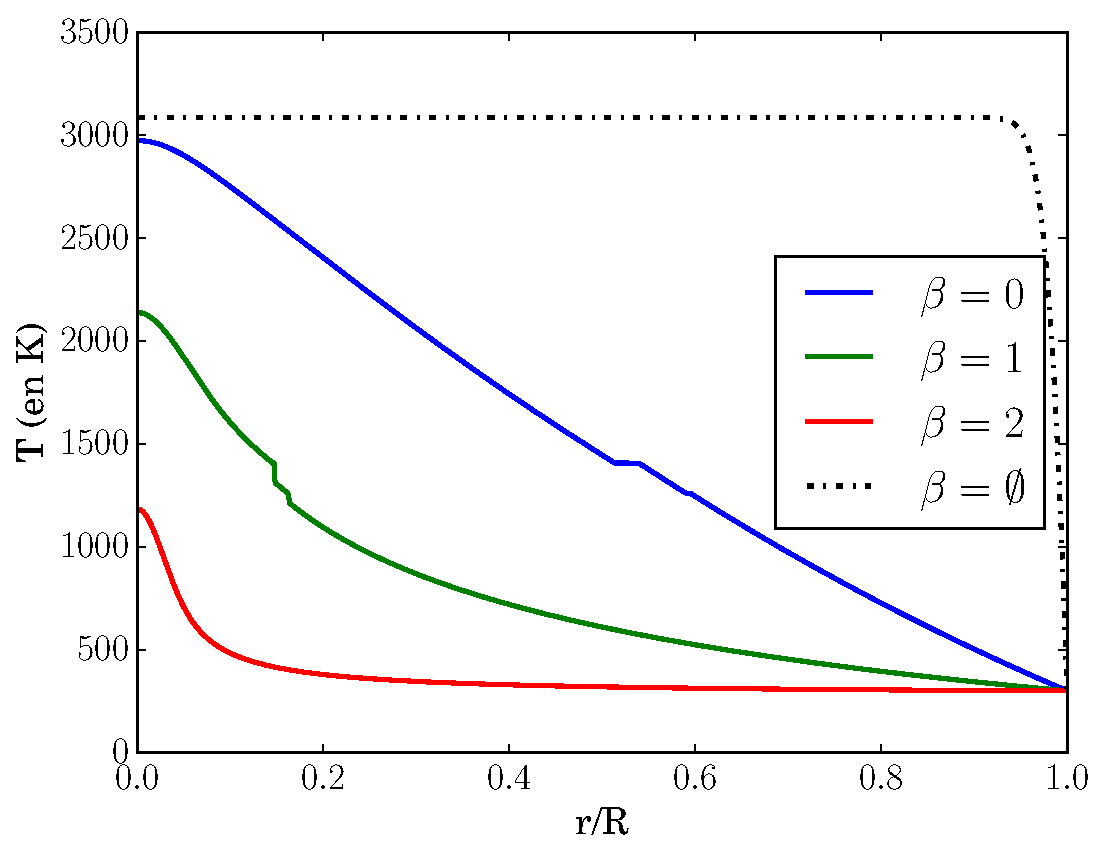
\includegraphics[scale=0.43]{figures/profil_acre.pdf}
    \caption{Profil de température à la fin de l'évolution d'un planétésimal de 5 à 500 km en 1 My. Le tracé en pointillés correspond au profil présenté en figure \ref{diffusion1} obtenu pour un astre de 500km après 1 My.}
    	\label{profilacre} 
\end{figure}

Dans le cas ou $\beta = 1$, un profil quasiment linéaire est observé et la température au centre est proche de celle observée pour un planétésimal de taille fixe. Le matériel étant ajouté relativement tôt dans l'histoire de la planète, il est encore capable de chauffer grâce à la radioactivité. 
\medskip

Pour $\beta = 1$ et 2, les températures sont nettement plus basse. Cela s'explique par le fait que la planète reste petite devant la longueur de diffusion pendant un temps long et tout le chauffage radioactif initial est évacué. La masse apportée à la fin de l'évolution  est moins efficace pour chauffer le planétésimal et n'a pas le temps de le faire, ce qui résulte en des températures sensiblement plus basses.


\subsection{Température moyenne au cours du temps}

Pour la suite, il peut être intéressant de s'intéresser à la température moyenne du planétésimal en fonction du temps. Ces courbes sont présentées en figure \ref{tempMoyacre}.

\begin{figure}[h]
    \centering	    
	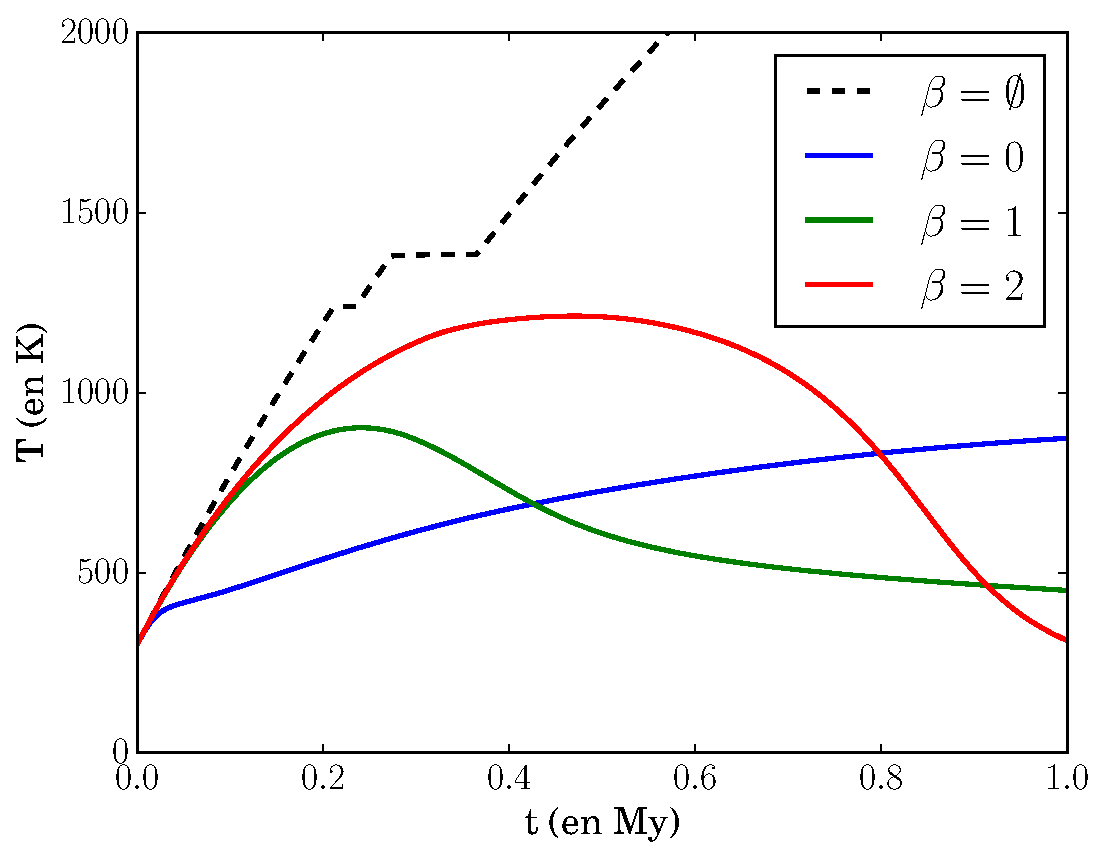
\includegraphics[scale=0.45]{figures/tempMoy_acretion.pdf}
    \caption{Température moyenne en fonction du temps pour l'évolution d'un planétésimal de 5 à 500 km en 1 My. Le tracé en pointillé correspond aux températures obtenues pour un astre de taille fixe égale à 500km.} 
    \label{tempMoyacre}
\end{figure}

Au début de l'évolution, les planètes évoluant avec un exposant $\beta= 1$ ou 2 sont les plus chaudes. Cela s'explique par le fait qu'elles récupèrent une petite quantité de matière leurs permettant de s'isoler en obtenant un rayon supérieur à la longueur de diffusion. Elles augmentent ensuite en température grâce au chauffage radioactif, sans être refroidi par la matière froide progressivement apportée de la surface par le terme d'accrétion. Cependant au fur et à mesure du temps, de plus en plus de masse est apportée et refroidit la planète.
\medskip

À l'inverse, pour $\beta = 0$, de la matière froide est apportée en plus grosse quantité dès le début de l'évolution. Cette matière va ensuite chauffer le planétésimal. La matière supplémentaire apportée continuellement de la surface vient cependant refroidir la planète en moyenne.
%%%%%%%%%%%%%%%%%%%%%%%%%%%%%%%%%%%%%%%%%%%%%%%%%%%%%%%%%%%%%%%%%%%%%%%%%%%%%%%%%%%%%%%%
%%%%%%%%%%%%%%%%%%%%%%%%%%%%%%%%%%%%%%%%%%%%%%%%%%%%%%%%%%%%%%%%%%%%%%%%%%%%%%%%%%%%%%%%
\section{Influence du chauffage par impact}
%%%%%%%%%%%%%%%%%%%%%%%%%%%%%%%%%%%%%%%%%%%%%%%%%%%%%%%%%%%%%%%%%%%%%%%%%%%%%%%%%%%%%%%%
%%%%%%%%%%%%%%%%%%%%%%%%%%%%%%%%%%%%%%%%%%%%%%%%%%%%%%%%%%%%%%%%%%%%%%%%%%%%%%%%%%%%%%%%
%%%%%%%%%%%%%%%%%%%%%%%%%%%%%%%%%%%%%%%%%%%%%%%%%%%%%%%%%%%%%%%%%%%%%%%%

\subsection{Prise en compte dans le modèle}
On considère maintenant l'ajout d'une source de chaleur supplémentaire qui est celle des impacts. L'énergie apportée provient de deux sources. La première est bien sûr l'énergie cinétique qui a été prise comme étant l'énergie gravitationnelle des impactants. Cette énergie correspond donc à l'énergie cinétique associé à la vitesse de libération de l'impactant. La seconde source d'énergie est l'énergie thermique propre des impactants. Pour évaluer la température de ces impactants et donc cette énergie, deux modèles ont été utilisés. Dans le premier, on considère que la température des impactants est de 1000K. Dans le second, on utilise le modèle précédent d'accrétion pour déterminer cette énergie : les impactants évoluent de la même manière que le planétésimal.
\medskip

Ensuite, seul $20\%$ de l'énergie de l'impact est effectivement transmise au planétésimal. Ce facteur permet de tenir compte du fait que le paramètre d'impact n'est pas toujours parfait, mais aussi du fait que, le choc ayant lieu à la surface, une grosse partie de l'énergie est directement perdue à la surface.
\medskip

Enfin, le rayon des impactant a été évalué à R/5 à l'aide de modèles statistiques d'agrégation et on a considéré que l'énergie était introduite sur cette profondeur.

Cette étude peut donc être résumée en 4 points :
\begin{enumerate}
\item La croissance est due à la masse apportée par les impactants
\item Seulement $20\%$ de l'énergie des impactants est introduite
\item L'énergie est répartie sur une couche d'épaisseur $R/5$
\item La température des impactants est de 1000 K ou déterminée par le modèle précédent.
\end{enumerate}

%%%%%%%%%%%%%
\label{impactant}
\subsection{Profil de température}

\begin{figure}[h]
    \centering	    
	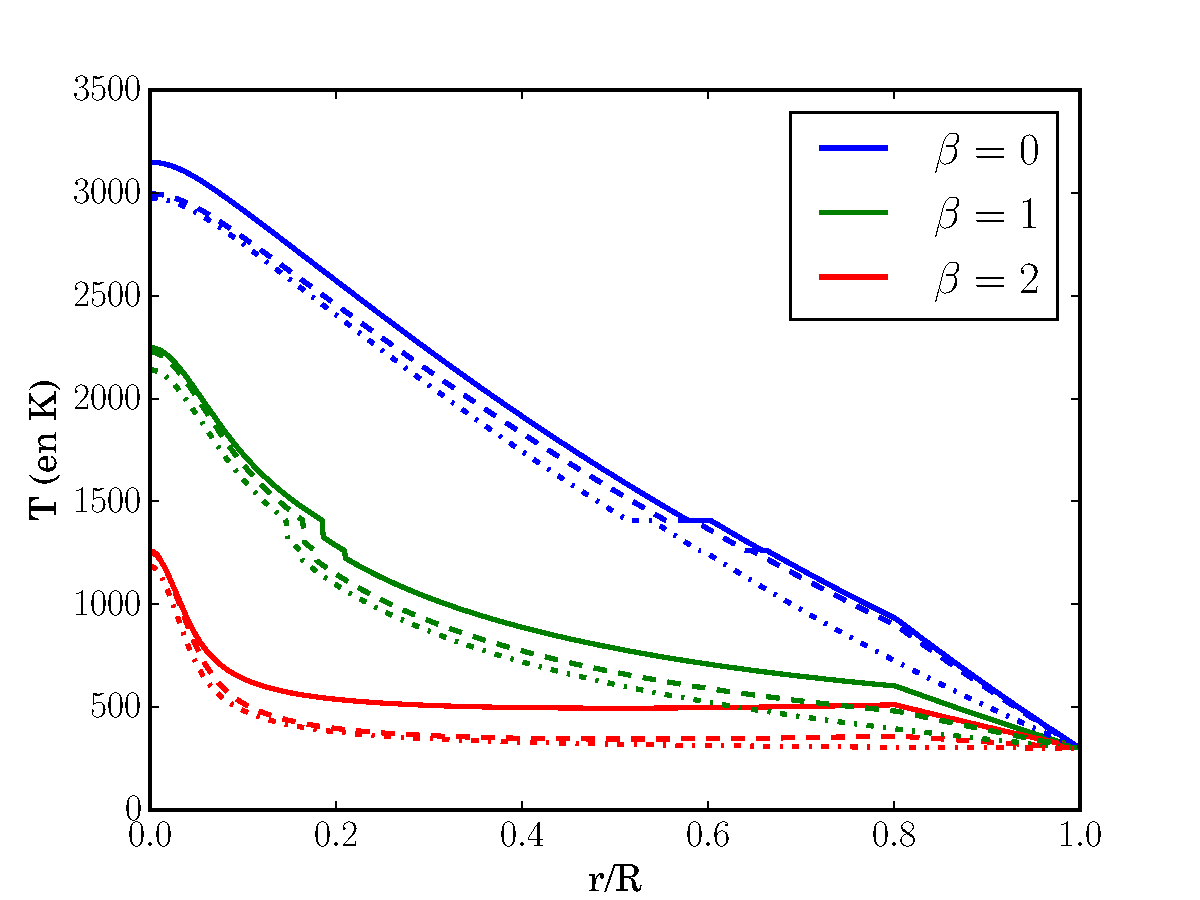
\includegraphics[scale=0.45]{figures/impact2.pdf}
    \caption{Profil de température à la fin de l'évolution d'un planétésimal de 5 à 500 km en 1 My. Le tracé en trait plein correspond à des impactants à 1000K. Le tracé en tirets correspond à des impactants dont la température est déterminée à l'aide du modèle d'accrétion simple.  Le tracé en pointillés correspond au profil présenté en figure \ref{profilacre} (sans impacts).}
    	\label{impact} 
\end{figure}

La figure \ref{impact} montre les résultats de cette étude. Le chauffage par des impactants de température 1000K implique une augmentation de la température de 200K par rapport au modèle d'accrétion simple. Ce comportement est observé pour les trois exposants $\beta$ utilisés.
\medskip

Le modèle complet considérant l'évolution en température des impactants donne cependant des résultats plus mitigés et l'augmentation n'est plus que de quelques dizaines de kelvin.
\medskip

Ainsi, l'importance du chauffage par impact pour les simulations est faible comparée à celle du chauffage radioactif et de l'accrétion. Cette dernière n'est pas suffisante pour permettre la création d'un noyau fondu la où il n'apparaît pas déjà. Bien entendu, comme on s'est intéressé aux planétésimaux au début de leur évolution, le chauffage radioactif prédomine. À l'inverse, si on s'intéresse aux temps longs, il est certain que le chauffage par impact devient la source principale d'énergie puisque la radioactivité diminue exponentiellement. 

%%%%%%%%%%%%%%%%%%%%%%%%%%%%%%%%%%%%%%%%%%%%%%%%%%%%%%%%%%%%%%%%%%%%%%%%%%%%%%%%%%%%%%%%
%%%%%%%%%%%%%%%%%%%%%%%%%%%%%%%%%%%%%%%%%%%%%%%%%%%%%%%%%%%%%%%%%%%%%%%%%%%%%%%%%%%%%%%%
\section{Conclusion}
%%%%%%%%%%%%%%%%%%%%%%%%%%%%%%%%%%%%%%%%%%%%%%%%%%%%%%%%%%%%%%%%%%%%%%%%%%%%%%%%%%%%%%%%
%%%%%%%%%%%%%%%%%%%%%%%%%%%%%%%%%%%%%%%%%%%%%%%%%%%%%%%%%%%%%%%%%%%%%%%%%%%%%%%%%%%%%%%%
%%%%%%%%%%%%%%%%%%%%%%%%%%%%%%%%%%%%%%%%%%%%%%%%%%%%%%%%%%%%%%%%%%%%%%%%
En conclusion, on a pu étudier l'influence des différents termes apparaissant dans le modèle gouvernant l'évolution en température d'un planétésimal. Cette étude permet de mieux comprendre les conditions dans lesquelles un noyau liquide peut se former. L'hypothèse de départ stipulant que le chauffage par impact joue un rôle important dans la différentiation est cependant fausse. En effet, la formation ou non du noyau est déterminée par la vitesse de croissance du planétésimal. On peut cependant nuancer nos propos en remarquant que le chauffage par impact est néanmoins responsable d'une nette augmentation de température sur l'intégralité du planétésimal et que ce dernier prédominera aux temps longs auxquels on ne s'est pas intéressé.


\newpage
\bibliographystyle{unsrt}
\bibliography{rapport} 
\addcontentsline{toc}{section}{Références} 


\end{document}
